\chapter{Reviews}
\label{vl:tc-review}

\dword{jpo} and \dword{tc} review all stages of detector development
and work with each consortium to arrange reviews of the design
(\dword{cdrev}, \dword{pdr} and \dword{fdr}), production (\dword{prr}
and \dword{ppr}), installation (\dword{irr}) and operation
(\dword{orr}) of their system. The reviews are organized by the
\dword{jpo} Review Office. In parallel the Review Office reviews all
stages of \dword{lbnf} cryostat and cryogenics development.  These
reviews provide information to the \dword{tb}, \dword{exb}, and \dword{efig}
in evaluating technical decisions. A timeline for the review process
is shown in Figure~\ref{fig:review_timeline}.
\begin{dunefigure}[DUNE review process]{fig:review_timeline}
  {\dword{dune} review process and timeline}
  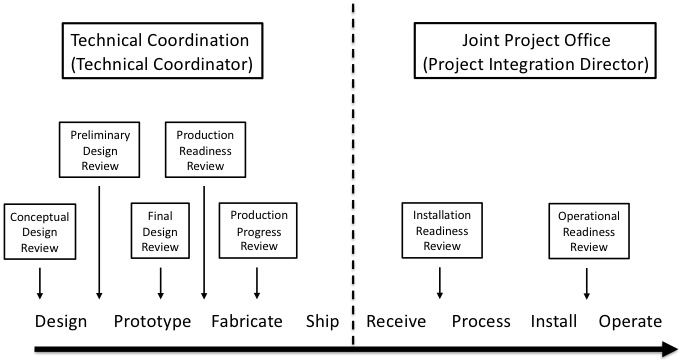
\includegraphics[width=0.75\textwidth]{review_timeline}
\end{dunefigure}
Review reports are tracked by \dword{jpo} and \dword{tc} and provide
guidance on key issues that require engineering oversight by the
\dword{jpo}/\dword{tc} engineering team. The Review Office maintains a
calendar of \dword{dune} reviews. The calendar of reviews is developed
by the Review Office in consultation with the \dword{ipd},
\dword{tcoord}, \dword{lbnf} project manager, consortia leads and
\dword{lbnf} subsystem managers.

\dword{tc} works with consortia leaders to prepare for reviews of all detector
designs.  As part of the \dword{tdr} development \dwords{pdr} were
arranged for many subsystems in advance of the \dword{tdr}. Some
remaining subsystem \dwords{pdr} will occur after the \dword{tdr}. All
subsystems will undergo \dwords{fdr}.  All major technology decisions
will be reviewed before down-select.  \dword{tc} may form task forces
as needed to address specific issues that require more in depth
review.


\dword{tc} works with consortia leaders to prepare for review of
detector component production processes.  Production of detector
elements begins only after successful \dwords{prr}. Regular production
progress reviews will be held once production starts depending on the
length of the production process. The \dwords{prr} will typically
include a review of the production of \textit{Module 0}, the first
module produced at the facility. \dword{tc} will work with consortia
leaders on all production reviews.

\dword{jpo} works with consortia leaders to prepare for review of
detector installation processes.  \dword{jpo} works with consortia
leaders to prepare for review of the installed detector components and
insure that they are ready for operations.  \dword{tc} coordinates
technical documents for the \dword{lbnc} \dword{tdr} review.

The review process is an important part of the \dword{dune} \dword{qa}
process as described in Section~\ref{sec:verification}, for
design and production.

The review process has been in place since 2016 with various reviews
of \dword{protodune} components and has continued into the first
\dword{dune} reviews in 2018--19. Past and scheduled reviews are in
the \dword{dune} Indico at https://indico.fnal.gov/category/586.
Review reports are currently maintained in~\citedocdb{1584}.

\section{Design Reviews}

The \dword{dune} design review process is described
in~\citedocdb{9564}. An updated mandate for the Review Office is under
development at EDMS-2173197\cite{bib:cernedms2173197}. Design reviews
for \dword{protodune} were held for each major system. Because the
schedule was extremely tight for \dword{protodune}, only a single
design review was held for each major system. Similarly a single
\dword{prr} was held for each major system.

The successful operation of \dword{protodune} means \dword{dune} is at
a very advanced state of design. The strategy going forward has been
to hold \dword{cdrev} for systems with significant changes from
\dword{protodune}. These systems include the \dword{dss}, \dword{pds},
\dword{daq} and calibration. These are systems that require changes
due to the size difference between \dword{protodune} and \dword{dune}
or the fact that one is in a test beam and one is underground. All
systems will go through \dwords{pdr} to review design changes from
\dword{protodune} and \dwords{fdr} after the \dword{tdr}.

\dword{tc} has established an Engineering Safety Committee with
mechanical and electrical engineering experts from collaborating
institutions to develop processes and procedures to evaluate
engineering designs using accepted international safety standards. The
current status of international code equivalencies is discussed
further in Section~\ref{sec:esh_codes}. The codes and standards to
which each system is designed will be reviewed as part of the
\dword{pdr} and \dword{fdr}.

\section{Production Reviews}

Once the designs are finished, production reviews will be held before
significant funds are authorized for large production runs. These
reviews are closely coordinated with the \dword{qa} team. The
expectation is that a \textit{Module 0} be produced and presented as
part of the \dword{prr}. The \textit{Module 0} is the first articles
from the production line and provide a useful indication of the
validity of production processes, time estimates and quality of the
product.

Once production has started, the Review Office will schedule \dwords{ppr} as
appropriate to monitor production schedule and quality. These reviews
will consist of site visits and will include membership from the
\dword{esh} and \dword{qa} teams.

The \dword{prr} process was exercized during \dword{pdsp}
construction. Because the schedule was extremely tight for
\dword{protodune}, only a single \dword{prr} was held for each major
system and no \dwords{ppr} were held.


\section{Installation Reviews}

\dwords{irr} are planned to verify equipment and procedures are in
place prior to installation of detector components. These will
review \dword{qc} results to verify that as-built detector
components can be successfully installed and operated. A critical part
of these reviews is to establish and verify the \dword{ha} for the
installation activities and mitigate any identified safety risks.  These reviews
will include safety personnel from \dword{surf} and \dword{fnal} as
appropriate.


\section{Operations Reviews}

\dwords{orr} will be organized by the Review Office before equipment
can be operated.  These serve as the final safety check out after
equipment has been installed and before it can be operated. These
reviews will include safety personnel from \dword{surf} and
\dword{fnal} as appropriate.

\section{Review Tracking}

Tracking and controling review recommendations is part of the review
process. Review committees assess recommendations from earlier
reviews. The Review Office assures that consortia respond to review
recommendations and works with the consortia to make sure the
responses are appropriately documented and implemented. Reports from
\dword{dune} reviews are maintained in~\citedocdb{1584} along with the
list of recommendations. The Review Office reports to the \dword{ipd},
\dword{tcoord}, and \dword{lbnf} project manager on recommendations
and progress towards completing actions on these recommendations.


%%%%%%%%%%%%%%%%%%%%%%%%%%%%%%%%
\section{Lessons Learned}
\label{sec:fdsp-coord-lessons}

A detailed list of lessons learned from construction and operation of
\dword{pdsp} is in~\citedocdb{8255}. These lessons have driven planning for
\dword{dune} and have led to design changes in \dword{dune}. Lessons
learned will continue to be updated throughout design review process
and into production. The methodologies are described in
Section~\ref{sec:quality_improvement}. %{sec:lessons_learned}.


%%%%%%%%%%%%%%%%%%%%%%%%%%%%%%%%
\section{Reporting}
\label{sec:fdsp-coord-reporting}

The \dword{dune} project has published regular monthly reports since
the final design and construction of \dword{protodune} began in
earnest in summer 2016. \dword{tc} currently plans to continue to compile and
publish these reports. The \dword{dune} project provides
regular reports to the \dword{lbnc} at reviews several times a
year. The \dword{jpo} Review Office produces reports from design,
production, installation and operations reviews.
